

\documentclass{article}
%\documentclass[10.8pt, a4paper, USenglish, twocolumn]{article}

%
%%%% DEPENDENCIES v1.7 %%%%%%

\usepackage{graphicx}
\usepackage[backend=bibtex,style=numeric,natbib=true,citestyle=numeric-comp,sorting=none]{biblatex}

\usepackage{amsmath}
\usepackage{amsthm}
\usepackage{amsfonts}
\usepackage{mathtools}
%\usepackage{enumerate}
\usepackage{enumitem}
\usepackage{todonotes}
\usepackage{esint}
\usepackage{float}
%
%\usepackage{mathrsfs}

\usepackage{hyperref}
\hypersetup{
    colorlinks=true, %set true if you want colored links
    linktoc=all,     %set to all if you want both sections and subsections linked
    linkcolor=blue,  %choose some color if you want links to stand out
}
\hypersetup{linktocpage}


% inscape-figures
%\usepackage{import}
%\usepackage{pdfpages}
%\usepackage{transparent}
%\usepackage{xcolor}
%\newcommand{\incfig}[2][1]{%
%\def\svgwidth{#1\columnwidth}
%\import{./figures/}{#2.pdf_tex} } \pdfsuppresswarningpagegroup=1

% Box environment
\usepackage{tcolorbox}
\usepackage{mdframed}
\newmdtheoremenv{definition}{Definition}[section]
\newmdtheoremenv{theorem}{Theorem}[section]
\newmdtheoremenv{lemma}{Lemma}[section]
\newmdtheoremenv{corollary}{Corollary}[section]

\DeclareMathOperator{\atantwo}{atan2}
\DeclareMathOperator{\arctantwo}{arctan2}


\theoremstyle{remark}
\newtheorem*{remark}{Remark}
%\newtheorem{example}{Example}

\newcommand{\newpara}
    {
    \vskip 0.4cm
    }

\usepackage{geometry}
%\usepackage{showframe} %This line can be used to clearly show the new margins

\newgeometry{vmargin={15mm}, hmargin={12mm,17mm}}

\addbibresource{bibliography.bib} % Makes the bibliography file available to biblatex.

%%%%%%%%%%%%%%%%%%%%%%%%%%%%%%%%%%%%%%%%%%%%%%%%%%%%%%%%%%%%
%
\title{Project Thesis\\Bananas and Troika}
\author{Isak Hammer }
\date{\today}
\begin{document}
    \begin{titlepage}
        \maketitle
        \begin{figure}
        \centering
        
\includegraphics[width=0.5\textwidth]{figures/front_page/dog.jpg}\\
        \end{figure}
        \thispagestyle{empty}
    \end{titlepage}

    \newpage
    \label{sec:eyyy}

    \section{Introduction}\label{sec:introduction}


The biharmonic equation is a fourth order partial differential equation which has gained great importance in
application such as mathematical modelling of linear elastic theory \cite{selvadurai13} and phase separation mechanics
of two phase systems \cite{cahnhilliard1957, kim16}. However, methods for solving the biharmonic equation analytically
is considered extensive and often impossible. Even on very simple plane problems on a unit square often requires advanced computations using integral transforms, variable separations, complex analysis and more \cite{selvadurai13}. We therefore tend
to lean towards approximating the solution using numerical methods for complicated problems.

There is generally two classes of numerical methods to solve the biharmonic equation. The first class is known as finite difference method (FDM) \cite{geer06,ehrlich75, hackbusch17}. Nevertheless, FDM does not handle complex domains well since it generally has strict requirements for the mesh generation. However, some methods have been introduced to solve problems on irregular domains, but is has shown to be relative extensive to implement \cite{hackbusch17, chen08, belyaev18}.

The second class is denotes as finite element method (FEM). Using this methods implies that there is theoretically no difference on solving problems on a regular or irregular domains, except for taking account for numerical stability and some
restrictions on mesh generation \cite{chen08}. However, a major challenge in FEM is to choose a discrete solution space on the finite elements to approximate the exact solution. We say that a method is conforming if the discrete solution space
$V_{h}$ is subspace of the exact solution space $V$, i.e. $V_{h} \subseteq  V$ \cite{shi02, brenner07math}. In general, for conforming methods requires that for a problem of order $2n$ must the discrete solution space be at least of order $n-1$. Thus, for a biharmonic problem
will a conforming FEM method demand at least a basis that is $C^1$ globally \cite{shi02}. From this strong continuity conditions rises a lot of complexity when constructing a finite element. In fact, attempts to solve this problems has shown that it
arise 21 degrees of freedom in a triangular Argyris element \cite{nair21}.

For nonconforming methods, $V_{h} \not \subseteq  V_{h}$ is the $C^{1}$ requirement completely relaxed. This makes the methods more suitable for forth order problems with the cost of more extensive error analysis. In fact, designing nonconformal
elements that does converge is rather difficult \cite{shi02, nair21}.

A third approach of FEM to solve the biharmonic equation is to solve the problem doing a mixed FEM method. This method seems promising, because it only requires $C^{0}$ elements \cite{chen08, brezzi91}.
Though this work well from a numerical point of view it has shown to have drawbacks by replacing symmetric positive definite continuous problem
by a saddle point problem, which is certainly makes the existence and uniqueness proof more challenging \cite{brezzi74}.

In this report will we focus to work on a fourth approach known as the continuous interior penalty method (CP). A major advantage is that the approach preserves the global $C^{0}$ continuity and the positive symmetric definiteness, thus makes it attractive to solve the biharmonic equation \cite{brenner2012, brenner2012quadratic}. In this report will we focus on presenting the derivation of CP and carry out a basic error analysis. We will also present a numerical analysis.


\section{Mathematical Background}%
\label{sub:mathematical_background}

In this section will we briefly establish some basic results of functional analysis and numerical analysis in order to construct the foundations of the FEM method. However, for a more thoroughly explanation some recommended sources are
\cite{brenner07math,manzoni2021optimal, quartdiff}. We will first define basic principles of Hilbert spaces which then will be applied to establish a theory for weak formulations the notion of a well-posed problem. Moreover, we will then continue by
establishing error estimates and constructing a numerical discretization of the weak formulation using a simple test problem.

\subsection{Hilbert Spaces}%
\label{sub:hilbert_spaces}

Assume $\Omega $  to be a compact and open set in $\mathbb{R} ^{2}$ and the parameter $p \in \mathbb{R} $, $p\ge 1$. We define $L^{p}\left( \Omega  \right) $ to be the set of all measurable functions $f: \Omega  \mapsto \mathbb{R} $ such that
$\left\lvert f \right\rvert ^{p}$ is Lebesgue measurable, i.e,

\begin{equation*}
    L^{p}\left( \Omega  \right) = \left\{ f: \Omega \mapsto \mathbb{R}  \mid \int_{\Omega }^{} \left\lvert f \right\rvert ^{p} d \Omega  < \infty  \right\}
.\end{equation*}

A useful extension which we will use later are the set of locally integrable functions such that for any compact subset $K \subseteq \text{Interior}\left( \Omega  \right) $, that is

\begin{equation*}
    L_{loc}^{1}\left( \Omega  \right)  = \left\{ f: f \in L^{1}\left( \Omega  \right)  \quad \forall K  \right\}.
.\end{equation*}


Let $u \in L^{p}\left( \Omega  \right) $, then we define the integral norm of order $p$ to be \[
\| u \|_{ L^{p}\left( \Omega  \right)  }^{  }  = \left( \int_{\Omega }^{} \left\lvert u \right\rvert ^{p} dx  \right) ^{\frac{1}{p}}
\]

Since $p=2$ is very frequently used we also define a more compact notation $\| u \|_{ \Omega  }^{  }  = \| u \|_{ L^{2}\left( \Omega  \right)  }^{  } $ .  We say that $L^{2}\left( \Omega  \right) $ is a Hilbert space if it is equipped with a inner
product of two functions $u,v \in L^{2}\left( \Omega  \right) $ such that
\[
\left( u,v \right) _{\Omega } = \left( u,v \right) _{L^2\left( \Omega  \right) } = \int_{\Omega }^{} u \cdot v dx
\]

In this report will we use the notation $\mathcal{V} $ for arbitrary Hilbert space. Note that we also use the notation $V^{*}$ for the dual space.

We will now establish a nation of the weak derivative, but first are we going to characterize some useful definitions of continuity. The space $C^{k}\left( \Omega  \right) $ for $k\ge 0$ denotes the set of functions whose derivatives, up to order of
$k$ , is continuous in $\Omega $. Note that we often use the shorthand notation \[
C^{0} = C\left( \Omega  \right)  = C^{0}\left( \Omega  \right)
\]
From this definitions we let $C^{\infty}\left( \Omega  \right) $ be the set of infinitely differentiable functions in $\Omega $ such that the space $C^{\infty}_{0}\left( \Omega  \right)$ is the set of all functions $u \in C^{\infty}\left( \Omega
\right) $ which is vanishing outside of any compact subset of $\Omega $. Let $u,v \in  C^{1}\left( \Omega  \right) $ and $\Gamma  = \partial \Omega $ with corresponding outer normal vector $n$, then this partial integration formula holds

\[
\int_{\Omega }^{} \nabla u \cdot v dx = \int_{\Gamma }^{} u\cdot v n ds - \int_{\Omega }^{} u \cdot \nabla v dx
\]

We now use this notation for derivatives \footnote{In literature is often $D^{\alpha } f$ commonly used, but later in the report is this notation reserved for the Hessian operator. }, $f \in C^{\left\lvert \alpha  \right\rvert } \left( \Omega  \right) $ so \[
\partial _{\alpha  } f = \frac{\partial ^{\left\lvert \alpha  \right\rvert } f}{ \partial ^{\alpha _{1} } x_{1} \partial ^{\alpha _{2}} x_{2}  }, \quad \alpha=\left( \alpha _{1}, \alpha _{2} \right)
\]


Finally, let $u \in  L^{1}_{loc}\left( \Omega  \right) $. We call the function $w \in L_{loc}^{1}\left( \Omega  \right) $ the $\alpha $-th weak derivative of $u$  if \[
\int_{\Omega }^{} w \varphi  dx = \left( -1 \right) ^{\left\lvert \alpha  \right\rvert } \int_{\Omega }^{} u \cdot \partial _{\alpha } \varphi dx, \quad \forall \varphi \in  C_{0}^{\infty}\left( \Omega  \right)
\]

Using the definitions introduced in this subsection can we construct the Sobolev space $H^{m}\left( \Omega  \right) , m>1$ , \[
H^{m}\left( \Omega  \right) = \left\{ u \in L^{2}\left( \Omega  \right)  \mid  \partial _{\alpha } u \in L^{2}\left( \Omega  \right)  \forall \alpha : \left\lvert \alpha  \right\rvert  \le m \right\}
\]

Equipped with the inner product is $H^{m}\left( \Omega  \right) $  denoted as a Hilbert space, that is, for $u,v \in H^{m}\left( \Omega  \right) $ is \[
    \left( u,v \right) _{H^{m}\left( \Omega   \right) } = \sum_{\left\lvert \alpha  \right\rvert  \le  m}^{}  \int_{\Omega }^{} \partial _{\alpha } u \partial _{\alpha } v dx.
\]

Similarly the integral norm is \[
\| u \|_{ H^{m}\left( \Omega  \right)  }^{  }  = \left( \| u \|_{ L^{2}\left( \Omega  \right)  + \sum_{k = 1}^{m}  \left\lvert u \right\rvert ^{2}  }^{  H^{k}\left( \Omega  \right) }  \right) ^{\frac{1}{2}}
\]
where the seminorm is define such that \[
\left\lvert u \right\rvert _{H^{k}\left( \Omega  \right) } = \left( \sum_{\left\lvert \alpha  \right\rvert  = k}^{} \| \partial _{\alpha }u \|_{ \Omega  }^{ 2 }  \right).
\]

We may also entitle the notation $H^{m}_{0} \left( \Omega  \right) = H^{m} \left( \Omega  \right) \cap C^{\infty}_{0} \left( \Omega  \right) $.





\subsection{Weak Formulation}%
\label{sub:weak_formulation}

By applying the theory in the previous subsection can we use describe the notion of a so-called weak formulation. Let us consider the simplest case, that is the strong form of the Poisson's equation with homogeneous Dirichlet boundary conditions
\begin{equation}
\label{eq:poisson_strong}
\begin{split}
-\Delta u & = f \quad \text{in } \Omega \\
u & =0 \quad \text{on } \partial \Omega
\end{split}
.\end{equation}

We want to obtain the weak formulation of the problem \eqref{eq:poisson_strong}. Let the trial function be $u \in H_{0}^{1}\left( \Omega  \right) $, then by integrating with a test function we get \[
\int_{\Omega }^{} - \Delta u \cdot v dx = \int_{\Omega }^{} f \cdot v dx \quad \forall v \in H^{1}_{0}\left( \Omega  \right)
\]
By using the partial integration formula and take the advantage of homogeneous Dirichlet boundary conditions the equation is in fact simplified to \[
a\left( u,v \right) = \int_{\Omega }^{}  \nabla u\cdot \nabla v dx , \quad l\left( v \right)  = \int_{\Omega }^{}  f\cdot v dx
\]

Hence, the final weak formulation has a symmetric bilinear form, $a\left( \cdot ,\cdot  \right) $, and a linear functional, $l\left( \cdot  \right) $, where we want to find a solution $u \in H^{1}_{0}\left( \Omega  \right) $  so

\begin{equation}
\label{eq:poissons_weak_formulation}
a\left( u,v \right) = l\left( v \right) \quad \forall v \in H^{1}_{0}\left( \Omega  \right).
.\end{equation}

We now want to establish that problems on this form is well-posed.
Lax-Milgram Theorem says that if we assume a Hilbert space $\mathcal{V} $ and the bilinear symmetric problem where we want to find a $u \in \mathcal{V} $  such that

\begin{equation*}
    a\left( u,v \right)  = \left( F, v \right) _{\mathcal{V} ^{*}, \mathcal{V} }, \quad \forall v \in  \mathcal{V}
.\end{equation*}

 Assuming the bilinear form $a\left( \cdot ,\cdot  \right) $  is continuous and coercive, i.e., the two conditions below.

\begin{enumerate}[label=\arabic*)]
    \item There exists a constant $M>0$ s.t. \[
    \left\lvert a\left( v,w \right)  \right\rvert \le M \| v \|_{ \mathcal{V}  }^{  } \| w \|_{ \mathcal{V}  }^{  }  \quad \forall v,w \in \mathcal{V}.
    \]
\item There exists a $\alpha  > 0$  so \[
a\left( v,v \right)  \ge  \alpha \| v \|_{ \mathcal{V}  }^{ 2 }.
\]
\end{enumerate}

We can then say there exists a unique solution $u \in \mathcal{V} $ and in additions it satisfied the stability estimate \cite{manzoni2021optimal}, \[
\| w \|_{ \mathcal{V}   }^{  } \le  \| F \|_{ V^{*} }^{  }
\]
Problems that fulfills this criteria is said to be well posed.


We can clearly see that this theorem applied to the weak formulation \eqref{eq:poissons_weak_formulation} since,
\[
\begin{split}
    \left\lvert a\left( v,w \right)  \right\rvert & \le \| \nabla v \|_{ \Omega  }^{  } \| \nabla w \|_{ \Omega  }^{  }, \\
\left\lvert a\left( v,v \right)  \right\rvert  & = \|  \nabla v\|_{\Omega   }^{  }  \| \nabla v  \|_{\Omega   }^{  } \ge  \| v \|_{ \Omega  }^{ 2 } \ge \| v \|_{ H^{1}\left( \Omega  \right)  }^{  }.
\end{split}
\]

On the last inequality was the Poincare inequality applied, i.e., there exists a $C>0$  such that $\| u \|_{ \Omega  }^{  } \le C  \| \nabla u \|_{\Omega   }^{  } $.


\subsection{Ceas' Lemma}%
\label{sub:ceas_lemma}

Since we have established a theory of a well-posed weak formulation we can now transition to setup a theory for a approximate solution. Assume that we have a problem that satisfied the Lax-Milgram theorem and let $\mathcal{V} _{h} \subseteq  \mathcal{V} $  be
some finite dimensional subspace of $\mathcal{V} $ such that $dim\left( \mathcal{V} _{h} \right) =N_{h}$ , where $h$  is a discretization parameter. The discretized problem is now to find a solution $u_{h} \in  \mathcal{V}_{h}$ such that $a\left( u_{h},v_{h} \right)  =
l\left( v_{h} \right) \quad  \forall v_{h} \in \mathcal{V} _{h} $. In fact, since the method is conform, i.e., $\mathcal{V} _{h} \subseteq  \mathcal{V} $ does it exists a exact solution $u \in  \mathcal{V} _{h}$ so, \[
a \left( u, v_{h} \right)  = l\left( v_{h} \right)  \quad  \forall v_{h} \in  \mathcal{V} _{h}.
\]

Using property can  we say that the problem is strongly consistent since it fulfills the Galerkin Orthogonality property, that is,  $ a\left( u -u_{h} , v_{h} \right)  =0$.

Now we have all the cornerstones for finding a error estimate . Again, assume that Lax-Milgram theorem holds. Let $v_{h} \in  \mathcal{V} _{h}$ so
\[
    \begin{split}
\alpha \| u -u_{h} \|_{ \mathcal{V}  }^{ 2 } & \le  a\left( u - u_{h}, u - u_{h}  \right)    \\
&= a\left( u - u_{h}, u -v_{h} \right) - a\left( u -u_{h}, v_{h} - u_{h} \right)  \\
\le  M \| u - u_{h} \|_{ \mathcal{V}  }^{  }  \| u - v_{h} \|_{ \mathcal{V}  }^{  }
    \end{split}
\]
Hence, the Ceas' lemma \cite{quartdiff} \[
\| u - u_{h} \|_{ \mathcal{V}  }^{  }  \le  \frac{M}{\alpha } \inf_{v_{h} \in \mathcal{V} } \|  v_{h} - u \|_{  }^{  }
\]

A useful property is that for a conformal numerical method to converge can we now only require \[
\lim_{h \to 0}  \inf_{v_{h} \in  V_{h}}  \| v - v_{h} \|_{ \mathcal{V }  }^{  } = 0 \quad  \forall v \in \mathcal{V}.
\]

In that case will $\| u - u_{h} \|_{ \mathcal{V}  }^{  }  \to  0$, $h \to  0$ .



\subsection{Finite Element Method}%
\label{sub:finite_element_method}
The idea of a conformal FEM method is to approximate a solution $\mathcal{V}_h \subseteq \mathcal{V}  $. However, the build blocks of the discretization relies on constructing a trianguation $\mathcal{T } _h$ with non-overlapping triangles  $T \in
\mathcal{T}_{h} $ so that \[
\Omega _{h} = Interior(\bigcup_{T \in  \mathcal{T} _{h}}^{} T) \implies \lim_{h\to 0} measure(\Omega - \Omega _{h}) = 0 \text{ a.e.}.
\]

For convenience will we generally use the notation $\Omega  = \Omega  _{h}$. We also denote the parameter $h$ as the diameter of the triangle $T$, i.e., $h_{T} = diam(T)$. Anyhow, this is later more precisely in the subsection
\ref{sub:computational_domain} later on, but for now does it hold as a basic introduction to conformal FEM.
Furthermore, let the space of finite elements suitable for our test problem in subsection \ref{sub:weak_formulation}, using the definition from \cite{quartdiff}, to be
\[
\mathcal{V} _{h} = \left\{ v_{h} \in C^{0}\left( \Omega  \right)  \mid  v_{h} \in \mathcal{P} _{r}\left( T \right)  \quad \forall T \in \mathcal{T} _{h}  \right\}
\]
where $\mathcal{P } _{r}\left( T \right) $ is the space of polynomials with degree $r$ for each $T$, that is,
\[
\mathcal{P} _{r}\left( T \right)  = \left\{ p\left( x_{1}, x_{2} \right) = \sum_{}^{i + j}  a_{ij} x^{i}_{1} x^{j}_{2}  \mid  a_{ij} \in \mathbb{R}  \text{ and } i,j \ge  0   \right\}.
\]

For the test problem can we observe that it is convenient to deal with a Lagrangian functions $\varphi _{j} \in V_{h}$, thus, for ever node $N_{u}$, \[
\varphi _{j}\left( N_{i} \right)  = \delta _{ij} = \begin{cases}
    0, \quad & i \neq j \\
    1,\quad & i=j
\end{cases}
\text{ where } i,j = 1,\ldots, N_{h}.
\]

Here is $N_{h}$  the total number of nodes which is chosen with caution. For the test problem, where $\Omega \subseteq \mathbb{R} ^{2} $, when $r=1$ is typically the nodes defined on the vertices and $ r=2 $ the nodes defined on the vertices and the
center of the edges/facets \cite{quartdiff}.
















    


\newpage
\section{Cahn Hilliard Equation on a Closed Membrane}%
\label{sec:cahn_hilliard_equation}


Let $c_0$ and $c_1$  indicate the concentration profile of the substances in a a $2$ -phase system such
that $c_0 \left( \mathbf{x},t \right): \Omega  \times \left[ 0, \infty \right] \to \left[ 0,1 \right]$ and
similarly $c_1 \left( \mathbf{x},t \right): \Omega \times \left[ 0, \infty \right] \to \left[ 0,1 \right]$, where
$\mathbf{x} $ is a element of some surface $\Omega $ and $t$ is time.
However, in the $2$ phase problem will we will restrict ourself so that $c_0\left( t,\mathbf{x} \right) + c_1\left( t,
\mathbf{x} \right) = 1$ at any $\mathbf{x} $ at time $t$. A property of the restriction is that we now can express
$c_0$ using $c_1$, with no loss of information. Hence, let us now define $c = c_0$ so $c \left( \mathbf{x},t \right):
\Omega  \times \left[ 0, \infty \right] \to \left[ 0,1 \right]$. It has been shown that $2$ phase system if
thermodynamically unstabl can be evolve
into a phase seperation
described by a evolutional differential equation \cite{cahnhilliard1957} using a model based on chemical energy of the
substances. However, further development has been done \cite{yushutin19} to solve this equation on surfaces. Now assume
model that we want to describe is a phase-seperation on a closed membrane surface $\Gamma $, so that $c \left( \mathbf{x},t \right):
\Gamma \times \left[ 0, T \right] \to \left[ 0,1 \right]$. Then is the surface Cahn Hilliard equation described such that

\begin{equation}
    \label{eq:cahn1}
\rho \frac{\partial c}{\partial  t}  - \nabla_{\Gamma } \left( M \nabla _{\Gamma } \left( f_{0}'  - \varepsilon ^2
        \nabla^2
_{\Gamma } c \right) \right) = 0  \quad \text{on } \Gamma
.\end{equation}

We define here the tangential gradient operator to be $\nabla _{\Gamma } c = \nabla c - \left( \mathbf{n} \nabla c
\right)\mathbf{n} $ applied on the surface $\Gamma $ restricted to $\mathbf{n} \cdot \nabla _{\Gamma } c = 0$.

Lets define $\varepsilon $ to be the size of the layer between the substances $c_{1}$ and $c_{2}$. The density $\rho $ is
simply defined such that $\rho = \frac{m}{S_{\Gamma }}$ is a constant based on the total mass divaded by the total
surface area of $\Gamma $.
Here is the mobility $M$ often derived such that is is dependent on $c$ and is crucial for the result during a possible
coarsering event \cite{yushutin19}.  However, the free energy per unit surface
$f_{0} = f_{0}\left( c \right)$ is derived based on the thermodynamical model and should according to \cite{yushutin19} be nonconvex and
nonlinear.

A important observation is that equation \eqref{eq:cahn1} is a fourth order equation which makes it more challenging to
solve using conventional FEM methods. This clear when writing the equation on the equivalent weak form and second order
equations arise.


\newpage
\section{Hybrid DG Method on HE}%
\label{sec:hybrid_dg_method_on_he}


Lets define the problem \[
\begin{split}
    -\varepsilon \nabla u &= f \quad \text{in } \Omega   \\
    u&= u_{D} \quad \text{on } \Gamma _{D} \\
    \partial _{n} u & = g \quad \text{on } \Gamma _{N} \\
    \partial _{n} u +  \beta u & = h \quad \text{on } \Gamma _{R}
\end{split}
\]
Here is $\partial \Omega  = \Gamma _{D} \cup \Gamma _{N} \cup \Gamma _{R}$. We want to write this on a weak form. Let
the spaces we work on be \[
    \begin{split}
H^{1}\left( \mathcal{T}_{h}  \right) & = \left\{ u \in L^2\left( \Omega  \right), u \in H^{1 } \left( T \right) \forall T
\in  \mathcal{T} _{h }\right\} \\.
    \end{split}
\]

For the problem to be discontinuous do we define the trial and test function to be $u \in H^{1 }\left( \Omega  \right) $

and $v \in H^{1 } \left( \mathcal{T} _{h} \right)$. Thus,
\begin{equation}
\label{eq:1a}
- \sum_{T \in \mathcal{T} _{h}}^{} \int_{ T}^{}   \varepsilon \nabla ^2 u \cdot v dx = \sum_{T \in \mathcal{T}_{h} }^{}
\left\{ \int_{T}^{} \varepsilon \nabla u \nabla v dx - \int_{\partial T}^{} \varepsilon\cdot  \partial _{n} u \cdot v ds
\right\} = \sum_{T \in \mathcal{T} _{h}}^{}  \int_{T}^{} f\cdot v dx
.\end{equation}

But we want to introduce the shorter notation equivalently such that
\begin{equation}
\label{eq:1b}
   \sum_{T \in \mathcal{T} _{h}}^{}
     \left\{ \varepsilon\left( \nabla u, \nabla v \right) _{T} -\varepsilon \left<\partial _{n} u,v \right>_{\partial T} \right\} = \sum_{T \in
  \mathcal{T} _{h}}^{}  \left( f,v \right)
.\end{equation}

Where $\left< \cdot ,\cdot  \right>$ is the surface integral operator. Before we contitinue do we want to introduce a
alternative method to integrate using edges. Let $v_{F} \in  L^2\left( \mathcal{F}_{h}  \right)$ for the set of all
facets $\mathcal{F} _{h}$. Now the surface integral can be rewritten such that
\begin{equation}
\label{eq:2}
    \begin{split}
 \sum_{T \in
\mathcal{T} _{h}}^{} \varepsilon  \left<\partial _{n} u , v_{F} \right>
&= \sum_{E \in \mathcal{F} ^{int}}^{}  \varepsilon \left<\partial _{n^{+}} u, v_{F} \right>_{E} + \varepsilon \left<
\partial _{n^{-}} u, v_{F}
\right>_{E} + \sum_{E \in \mathcal{F} ^{ext}}^{} \varepsilon \left<\partial _{n} u, v_{F} \right>   \\
    \end{split}
.\end{equation}

Lets define some crucial spaces for the DG method \[
    \begin{split}
V &=  \left\{ \left( u, u_{F} \right) : u \in H^2\left( \mathcal{T} _{h} \right) \cap H^{1}\left( \Omega  \right)   ,
u_{F} \in  L^2\left( \mathcal{F} _{h} \right)  \right\} \\
V_{h} &=  \left\{ \left( u,u_{F} \right) : u \in  \mathcal{P} ^{k} \left( T \right) \forall T \in  \mathcal{T} _{h} , \quad
u_{F} \in  \mathcal{P} ^{k}\left( E \right)  \forall E  \in \mathcal{F} _{h}   \right\} \\
    \end{split}
\]
and now including drichlet conditions using the previous definition \[
\begin{split}
    V_{D} & = \left\{ \left( u,u_{F} \right) \in V , u_{F} = u_{D} \quad  \text{on } \Gamma _{D}  \right\} \quad
    V_{h,D}  = \left\{ \left( u, u_{F} \right) \in  V_{h}, u_{F} = u_{D} \quad  \text{on } \Gamma _{D}  \right\} \\
    V_{0} & = \left\{ \left( u,u_{F} \right) \in V , u_{F} = 0 \quad  \text{on } \Gamma _{D}  \right\} \quad
    V_{h,0}  = \left\{ \left( u, u_{F} \right) \in  V_{h}, u_{F} = 0 \quad  \text{on } \Gamma _{D}  \right\}
\end{split}
\]

Defining  $\left( u, u_{F} \right) \in  V_{D} $ and $\left( v, v_{F} \right) \in  V_{0} $.
Now adding \eqref{eq:1b} and \eqref{eq:2} can we easily see that
\begin{equation}
    \label{eq:3a}
    \begin{split}
   \sum_{T \in \mathcal{T} _{h}}^{}
     \left\{ \varepsilon\left( \nabla u, \nabla v \right) _{T}  \right\}
     & = \sum_{T \in \mathcal{T} _{h}}^{}  \left( f,v \right) +\sum_{E \in \mathcal{F} ^{int}}^{}  \varepsilon \left<\partial _{n^{+}} u, v_{F} \right>_{E} + \varepsilon \left<
\partial _{n^{-}} u, v_{F} \right>_{E} + \sum_{E \in \mathcal{F} ^{ext}}^{} \varepsilon \left<\partial _{n} u, v_{F} \right>
    \end{split}
.\end{equation}

Applying the Neumann conditions on $ \Gamma _{N} $ and $\Gamma _{R}$, can the condition on the exterior facets
be rewritten such that
\[
\sum_{E \in \mathcal{F} ^{ext}}^{}  \varepsilon \left< \partial _{n} u, v_{F} \right> = \varepsilon \left<g,v_{F}
\right> _{\Gamma _{N}} + \varepsilon \left<h - \beta u, v_{F} \right> _{\Gamma _{R}}
\]
Keep in mind that we on the exterior boundaries define the integral so $\left<f, v_{F} \right> = \int_{\Gamma }^{} f
\cdot v_{F} \cdot n ds $ for a arbitary neumann boundary $f$ on some surface $\Gamma $. Hence \eqref{eq:3a} ends up
being
\begin{equation}
\label{eq:3b}
 \sum_{T \in \mathcal{T}_{h} }^{} \varepsilon \left( \nabla u , \nabla v \right)  - \sum_{E \in F^{int}}^{} \left(
\varepsilon  \left<\partial _{n^{+}} u , v_{F} \right> _{E} + \varepsilon \left<\partial _{n^{-}}  u, v_{F}\right>_{E}
\right) + \left<\beta u, v_{F} \right> _{\Gamma _{R}} = \sum_{T \in T_{h}}^{} \left( f,v \right)   + \left<g, v_{F}
\right>_{\Gamma _{N}} + \left<h, v_{F} \right>_{\Gamma _{R}}
.\end{equation}

According to Lehrenfeld 2010  \cite{lehrenfeld2010} at page 13 on equation (1.2.7)  is \eqref{eq:3b} equivalent to

\begin{equation}
\label{eq:3c}
\sum_{T \in \mathcal{T} _{h}}^{}   \left( \varepsilon \nabla u, \nabla v \right) _{T} -\sum_{T \in \mathcal{T} _{h}}^{}    \left<\varepsilon  \partial
_{n} u , \jump{ v } \right> _{\partial T}  + \beta  \left< \varepsilon u, v_{F}  \right>_{\Gamma _{R}} = \sum_{T
\in \mathcal{T} _{h}}^{} \left( f,v \right)  + \left<\varepsilon g, v_{F} \right>_{\Gamma _{N}} + \left<\varepsilon h,
v_{F} \right>_{\Gamma _{R}}
\end{equation}


Here is the jump defined simply as $\jump{v} = v - v_{F}$. Remember that $ v_{F} = tr_{\partial T} \left( v \right)  $. What we see is for \eqref{eq:3b} and \eqref{eq:3c} to be
equivalent must this be true.
\begin{equation}
\label{eq:3c2}
    \sum_{T \in \mathcal{T} _{h}}^{}  \left< \varepsilon \partial _{n} u, \jump{u}  \right>_{\partial T} = \sum_{T \in
    \mathcal{T} _{h}}^{}  \left< \varepsilon \partial _{n} u, u  \right>_{\partial T} - \left< \varepsilon
    \partial _{n} u, u_{F}  \right>_{\partial T} =\sum_{E \in
    \mathcal{F} ^{int}}^{}  \varepsilon \left( \left< \partial _{n^{+}} u, v_{F} \right>_{E}  + \left<\partial _{n^{-}}
u, v_{F}\right> \right)
.\end{equation}

\todo{why is it true??}


Since $\left( u, u_{F} \right) \in V $ is has to be continious, hence the jump $\jump{u} = 0$ for a good solution. Hence
we can add $-\left<\varepsilon \partial _{n} \jump{u} \right>_{\partial T}$ and $ \tau _{h} \left<\varepsilon \jump{u},
\jump{v} \right>_{\partial T}$ for each $T \in  \mathcal{T}_{h} $. We can add this to lhs on \eqref{eq:3c2} so



\begin{equation}
\label{eq:3c}
\begin{split}
    \sum_{T \in \mathcal{T} _{h}}^{}   \left( \varepsilon \nabla u, \nabla v \right) _{T} &-\sum_{T \in \mathcal{T} _{h}}^{}
\left\{ \left<\varepsilon  \partial
_{n} u , \jump{ v } \right> _{\partial T}  -\left<\varepsilon
\partial _{n} \jump{u} \right>_{\partial T}  + \tau _{h} \left<\varepsilon \jump{u},
\jump{v} \right>_{\partial T} \right\}  \\ &+ \beta  \left< \varepsilon u, v_{F}  \right>_{\Gamma _{R}} \\
                                           &= \sum_{T
\in \mathcal{T} _{h}}^{} \left( f,v \right)  + \left<\varepsilon g, v_{F} \right>_{\Gamma _{N}} + \left<\varepsilon h,
v_{F} \right>_{\Gamma _{R}}
\end{split}
\end{equation}









\section{$C^0$ Interior Penalty Method}
\label{sec:ch1}

\subsection{Introduction of the Boundary Value Problem}%
\label{sub:introduction_of_the_bvp}


In this section do we want to establish a numerical method to fourth order equations. Instead of embarking on the
special case of surface PDE described in \eqref{eq:cahn1} can we establish a general numerical theory on $\mathbb{R} ^2$, which we later can generalize on closed surface later. Assume that we restrict ourself to a compact surface $\Omega \in \mathbb{R} ^2 $ and let $f \in L^{2}\left( \Omega
\right) $ as defined in \ref{sub:l_2_space}.
Let say we want to solve the equation on the form.

\begin{equation}
\label{eq:ch1_bvp}
\begin{split}
    \Delta ^2 u - \beta \Delta u + \gamma u &= f \quad \beta , \gamma \ge 0 \\
    \frac{\partial u}{\partial  n}  &= 0 \quad \text{on }\Omega  \\
    \frac{\partial \Delta u}{\partial  n}  &= q \quad \text{on } \partial \Omega  \\
\end{split}
.\end{equation}

For convenience are the boundary condition $q$ chosen to be defined via a  $\phi \in H^{4}\left( \Omega  \right)$
such that $q = \frac{\partial \Delta \phi }{\partial  n} $ so $\frac{\partial \phi }{\partial  n}  = 0$.
$\partial \Omega $.


\subsection{Weak Formulation}%
\label{sub:weak_formulation}

We want to rewrite \eqref{eq:ch1_bvp} on weak formulation. Now define the Hilbert space \[
V = \left\{ v \in H^2\left( \Omega  \right): \frac{\partial v}{\partial  n}  = 0 \quad \text{on } \partial \Omega
\right\}.
\]
It can be shown \cite{gu2012c0} that a convinient form is to write it as
\begin{equation}
\label{eq:weakform}
    \begin{split}
a\left( u,v \right) &=  \left( f,v \right)_{L^2\left( \Omega  \right)}  - \left( q,v \right)_{L^2\left( \partial \Omega  \right)}  \\
& = \int_{\Omega }^{} D^2 w : D^2 v dx +  \int_{\Omega }^{} \nabla w \nabla v dx + \int_{\Omega }^{} \gamma w \cdot v dx
.\\
    \end{split}
.\end{equation}
For all $\forall v \in  V$, where \[
D^2 w : D^2 v = \sum_{i,j=1}^{2}  \frac{\partial ^2 w}{\partial x_{i} \partial x_{j} } \cdot  \frac{\partial ^2 v
}{\partial x_{i} \partial x_{j} }.
\]

% Abusing notation can we see this is clearly arise since \[
%     \begin{split}
% \int_{\Omega }^{} \Delta ^2 w \cdot  v   dx & = - \int_{\Omega }^{} \nabla \left( \Delta w \right) \nabla v dx \\
% &= \int_{\Omega }^{} \Delta w \Delta v dx  -\int_{\partial \Omega }^{} \nabla v \frac{\partial \Delta w}{\partial n } ds   \\
% &= \left( \Delta w, \Delta v \right)_{L^2\left( \Omega  \right)} - \left( q,v \right) _{L^2\left( \partial \Omega  \right)} \\
%     \end{split}
% \]
% \todo[inline]{ why is minus sign in front of $\left( q,v \right) _{L^2\left( \partial \Omega  \right)}$ and is it
% correct to use $q$ in this setting? I also wonder how  $ \left( \Delta w, \Delta v \right)$ appears to be $\left( D ^2
% w, D^2 v \right)$ at some point.}

In fact, according to \cite{gu2012c0} can it be shown that the problem has a unique solution if and only if $\gamma >
0$. However, in the case where $\gamma  = 0$ can we provoke a unique solution by introducing the condition \[
\int_{\Omega }^{} f dx = \int_{\partial \Omega }^{}  q ds
\]

Taking this into account can we expand the solution space such that \[
V^* = \begin{cases}
    V, \quad & \text{if } \gamma >0 \\
    \left\{ v \in V: v\left( p^* \right) = 0 \right\}, \quad & \text{if } \gamma  =0
\end{cases}
\]

Where $p^{*}$  is a corner in $\Omega $. In fact, now all solutions of \eqref{eq:weakform} exists in $V^{*}$.


\subsection{Construction of $C^{0}$ Interior Penalty Method}%
\label{sub:construction_interior_penalty_method}

We want to construct a $C^{0}$ interior penalty method based on $C^{0}$ Lagrange elements.
Assume $\mathcal{T}_{h} $ be a triangulation of $\Omega $ and $V_{h}$ be the à $\mathcal{P}_{2} $ Lagrange finite
element space associated with $\mathcal{T}_{h} $ \[
V_{h} = \left\{ v \in C\left( \overline{\Omega } \right) : v_{T} = v |_{T} \in \mathcal{P}_{2}\left( T \right) \quad
\forall T \in  \mathcal{T} _{h}  \right\}
\]
So that we can earn a similar space for the approximated solution space ,
\[
V_{h}^{*} = \begin{cases}
    V_{h}, \quad & \text{for } \gamma >0\\
    \left\{ v \in V_{h}: v\left( p^{*} \right) = 0 \right\} \quad & \text{for } \gamma = 0.
\end{cases}
\]
Here is $p^{*}$ again a corner in $\Omega $. Let us now generalize the Hilbert space as well to the approximated
solution space by defining \[
H^{k}\left( \Omega , \mathcal{T} _{h}  \right) = \left\{ H^{1}\left( \Omega  \right): v_{T} \in H^{k}\left( T
\right)\quad \forall T \in \mathcal{T} _{h} \right\}.
\]
\begin{figure}[!h]
\centering
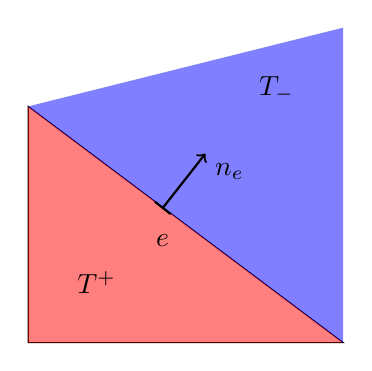
\begin{tikzpicture}[scale=1]
\coordinate (A) at (0,0);
\coordinate (C) at (0,3);
\coordinate (B) at (4,0);
\coordinate (D) at (4,4);
\coordinate (Tm) at (3.5,3.5);
\coordinate (Tp) at (0.5, 0.5);
\coordinate (e) at (1.5, 1.5);
\coordinate (start) at (1.7, 1.7);
\coordinate (end) at (2.25, 2.4);

\draw (A) -- (B) -- (C) -- cycle;
\fill[red, opacity=0.5] (A) -- (B) -- (C);
\fill[blue, opacity=0.5] (B) -- (C) -- (D);
\node[below left] at (Tm) {$T_{-} $ };
\node[above right] at (Tp) {$T^{+}$ };
\node[below right] at (e) {$e$ };

\draw [|->, thick] (start) -- (end);
% \node[above right] at (A) {A };
% \node[below right] at (B) {B};
% \node[above right] at (C) {C };
% \node[below right] at (D) {D};
\node[below right] at (end) {$n_e$};
\end{tikzpicture}
\caption{Edge $e$ shared by the triangles $T_{-}$ and $T_{+}$ and the normal unit vector $n_{e}$.  }
    \label{fig:normal}
\end{figure}

Now assume that that $e \in \mathcal{E}_{h}^{i} $ is shared between two triangles $T_{-}, T_{+} \in  \mathcal{T} _{h}$ .
Then we can assume that the unit normal from $T_{-}$ to $T_{+}$ is described as $n_{e}$ as illustrated in figure
\ref{fig:normal}. Finally, we now want to define jumps internally, \[
\begin{split}
    \jump{ \frac{\partial v_{h}}{\partial n_{e}} } &= \frac{\partial v_{T_{+}}}{\partial n_{e}  } | _{e} -
    \frac{\partial v_{T_{-}}}{\partial n_{e}  } |_{e}, \quad \forall v \in H^{2}\left( \Omega , \mathcal{T} _{h} \right)  \\
    \jump{ \frac{\partial ^2 v_{h}}{\partial n_{e} ^2 } } &= \frac{\partial ^2 v_{T_{+}}}{\partial  n_{e}^2} |_{e}  -
    \frac{\partial ^2 v_{T_{-}}}{\partial n_{e}^2   } |_{e} \quad \forall v \in H^3\left( \Omega , \mathcal{T} _{h}
    \right).  \\
\end{split}
\]

And similarly for means internally,
\[
    \begin{split}
\mean{ \frac{\partial v_{T_{-}}}{\partial n_{e} } } &= \frac{1}{2} \left( \frac{\partial v_{T_{+}}}{\partial n_{e} }
|_{e} +  \frac{\partial v_{T_{-}}}{\partial n_{e} } |_{e}  \right) \quad  \forall v \in H^2\left( \Omega , \mathcal{T}
_{h} \right) \\
    \mean{ \frac{\partial ^2 v_{h}}{\partial n_{e}^2 } } &= \frac{1}{2} \left( \frac{\partial ^2 v_{T_{+}}}{\partial
    n_{e}^2  } |_{e} + \frac{\partial ^2 v_{T_{-}}}{\partial n_{e}^2  } |_{e}    \right) \quad \forall v \in  H^3\left( \Omega .
\mathcal{T}_{h}  \right), \\
    \end{split}
\]

Let the edges along the boundary be defined as $e \in  \mathcal{E} _{h}^{b}$ along a some boundary triangle $\mathcal{T}
_{h}$. We can then define the jump and mean as \[
\begin{split}
    \jump{ \frac{\partial v_{h} }{\partial n_{e} } } & = -\frac{\partial v_{T}}{\partial  n_{e}} |_{e} \quad \forall v \in
    H^2\left( \Omega , \mathcal{T}_{h}  \right) \\
    \mean{ \frac{\partial ^2 v_{h}}{\partial n_{e}^2 } } & = \frac{\partial v_{T}}{\partial  n_{e}} |_{e} \quad \forall v \in
    H^3\left( \Omega  , \mathcal{T}_{h}  \right)
\end{split}
\]

Using the results from \cite{gu2012c0} can we formulate the discrete formulation the boundary value problem
\eqref{eq:ch1_bvp} using $C^{0}$ interior penalty method. Our goals is to find a $u_{h} \in V_{h}^{*} $ such that this
is true,

\begin{equation}
\label{eq:C0-methoda}
\mathcal{A} \left( u_{h}, v_{h}  \right) = \left( f, v_{h} \right)_{L^{2}\left( \Omega  \right)} - \left( q, v_{h}
\right) _{L^{2}\left( \partial \Omega  \right)} \quad  \forall v_{h} \in V_{h}^{*}
.\end{equation}

Where $w_{h}, v_{h} \in  V_{h}$ and
\begin{equation}
\label{eq:C0-methodb}
\begin{split}
    \mathcal{A} \left( w_{h}, v_{h} \right) &=  \sum_{T \in \mathcal{T} _{h}}^{} \int_{T}^{} D^2 w_{h} : D^2 v_{h}  \\
    & + \sum_{e \in  \mathcal{E} _{h}}^{} \int_{e}^{ } \mean{ \frac{\partial ^2 w _{h}}{\partial n_{e}^2 } } \jump{
    \frac{\partial v_{h}}{\partial  n_{e}} }  ds \\
    & + \sum_{e \in \mathcal{E} _{h}}^{} \mean{ \frac{\partial ^2
v_{h}}{\partial n_{e }^2 } } \jump{ \frac{\partial w_{h}}{\partial n_{e}} }  ds \\
 &  + \sum_{e \in \mathcal{E} _{h}}^{} \frac{\sigma }{\left\lvert e \right\rvert } \int_{e}^{} \jump{ \frac{\partial
 w_{h}}{\partial n_{e}}} \jump{ \frac{\partial v_{h}}{\partial n_{e}} } ds \\
 & + \int_{\Omega }^{}  \beta \nabla w_{h} \cdot \nabla v_{h} dx + \int_{\Omega }^{} \gamma w_{h} v_{h} dx .
\end{split}
.\end{equation}

The notation $\left\lvert e \right\rvert $ is to describe the length of the edge $e$ and $\sigma  \ge  1$ is a penalty
parameter.



    \printbibliography

\end{document}
